\section{Related Work}
\label{sec:related-work}
%%%%%%%%%%%%%%%%%%%%%%%%%%%%%%%%%%%%
\begin{figure*}[t] 
    \centering 
    \vspace*{-2mm}
    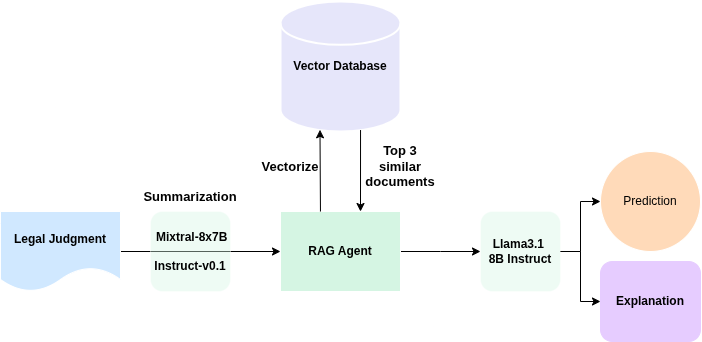
\includegraphics[width=0.75\linewidth]{figures/Generic_flow_chart.drawio.png} 
    \vspace*{-2mm}
    \caption{Illustration of our Legal Judgment Prediction framework using RAG. The input legal judgment is first summarized; a RAG agent retrieves top-3 relevant documents from a vector database; and an instruction-tuned LLM (e.g., LLaMA-3.1 8B Instruct) generates the final prediction and explanation.}
    \label{fig:task-framework}
\end{figure*}
%%%%%%%%%%%%%%%%%%%%%%%%%%%%%%%%%%%%
Recent advances in natural language processing (NLP) and large language models (LLMs) have transformed knowledge-intensive tasks, including question answering and decision support. Transformer-based architectures such as BERT \citep{devlin2018bert}, GPT \citep{radford2019language}, and their instruction-tuned successors demonstrate strong multi-hop reasoning and contextual generation abilities. Retrieval-Augmented Generation (RAG) further improves factual grounding and reduces hallucinations by combining external document retrieval with generative models \citep{han2024rag,hei2024dr}.

The domain of Legal Judgment Prediction (LJP) has evolved from outcome classification toward explanation generation and realistic reasoning. Foundational work explored case outcome prediction in ECHR and Chinese datasets \citep{aletras2016predicting, chalkidis2019neural, xiao2018cail2018}, inspiring subsequent benchmarks such as CAIL2018 and ECHR-CASES. Recent approaches have incorporated statutes, reasoning structures, and event-based features \citep{feng-etal-2022-legal, feng2023criminal}.

Within the Indian legal ecosystem, the ILDC corpus \citep{malik-etal-2021-ildc} laid the foundation for Court Judgment Prediction and Explanation (CJPE). This has been expanded in PredEx \citep{nigam2024legaljudgmentreimaginedpredex}, NyayaAnumana \citep{nigam2024nyayaanumana}, LegalSeg \citep{nigam2025legalseg}, TathyaNyaya \citep{nigam2025tathyanyaya}, and IBPS for bail prediction \citep{srivastava2025ibps}, which collectively focus on segmentation, factual reasoning, and judgment outcome explanation. Efforts such as \citep{nigam2024rethinking,10.1145/3632754.3632765} emphasize fact-based LJP as a realistic alternative to full-text reasoning, aligning predictions more closely with early-phase decision-making. Other works explore semantic segmentation \citep{malik2021semantic}, legal QA \citep{nigam2023legal}, and structured document generation \citep{nigam2025structured}. These resources and models highlight the significance of domain-specific adaptation for Indian law, an underrepresented common law system.

Precedent integration is central to common law reasoning. Early precedent-aware models such as \citep{zhao-etal-2018-learning} focused on Chinese law, while recent works like PLJP \citep{wu2023precedent}, LexKeyPlan \citep{santosh2025lexkeyplan}, and precedent-enhanced ECHR prediction \citep{santosh2024incorporating} examine retrieval of historical judgments to guide predictions. These align with broader multilingual and cross-jurisdictional LJP studies \citep{niklaus2021swiss, kapoor-etal-2022-hldc}. While these efforts highlight the role of past cases, their settings differ significantly from India’s unique common law context where both statutory law and judicial precedents guide reasoning.

Retrieval-augmented pipelines are increasingly applied to legal NLP. LegalBench-RAG \citep{pipitone2024legalbench} and CLERC \citep{hou2024clerc} introduced benchmarks for retrieval-augmented legal reasoning. Specialized systems like CBR-RAG \citep{wiratunga2024cbr}, Graph-RAG for norms \citep{de2025graph}, and LexKeyPlan \citep{santosh2025lexkeyplan} explore structured retrieval, case-based reasoning, and keyphrase-driven planning. Applications range from legal assistants and dispute resolution \citep{rafat2024ai,10887211} to federated secure access architectures \citep{amato2024optimizing}. These works demonstrate the value of augmenting generative reasoning with statutory and precedent-based retrieval but primarily address civil law or international corpora.

Our work contributes to this line by contextualizing RAG for the Indian common law system, simulating how judges reason with case facts, statutory provisions, and precedents. While prior RAG frameworks in law \citep{wiratunga2024cbr, hou2024clerc, wu2023precedent, santosh2024incorporating} establish the feasibility of retrieval-augmented pipelines, they have not been applied to Indian courts. By integrating factual, statutory, and precedential inputs in a unified framework, NyayaRAG extends the landscape of LJP toward realistic, explainable, and domain-grounded legal tasks.